\documentclass[a4paper,10pt,french]{report}
\usepackage[utf8]{inputenc}
\usepackage[left=4cm, right=4cm]{geometry}
\usepackage{pdfpages}
\usepackage[english,frenchb]{babel}
\usepackage[T1]{fontenc}


%librairie caractères spécion
\usepackage{hyperref}
\usepackage{lmodern}
\usepackage{amsmath}
\usepackage{amssymb}
\usepackage{mathrsfs}

%%librairie image flottant
\usepackage{wrapfig}

\usepackage{minted}

% librari landscape
\usepackage{lscape}

\renewcommand{\partname}{}
\renewcommand{\thechapter}{}
\renewcommand{\thesection}{}
\renewcommand{\appendix}{}
\renewcommand{\figurename}{Figure}
% numérotation des figures
\renewcommand{\thefigure}{\Roman{part}.\arabic{figure}}

\usepackage{glossaries}
\makeglossaries

\makeatletter
\title{Solution d'acquisition et de stockage de données et étude sur l'anonymisation de données} \let\Title\@title
\author{Bertrand NDAYISENGA} \let\Author\@author
\date{2017-2018} \let\Date\@date

\begin{document}

    %page de garde
    %%%% debut macro %%%%
\newenvironment{changemargin}[2]{\begin{list}{}{%
\setlength{\topsep}{0pt}%
\setlength{\leftmargin}{0pt}%
\setlength{\rightmargin}{0pt}%
\setlength{\listparindent}{\parindent}%
\setlength{\itemindent}{\parindent}%
\setlength{\parsep}{0pt plus 1pt}%
\addtolength{\leftmargin}{#1}%
\addtolength{\rightmargin}{#2}%
}\item }{\end{list}}
%%%% fin macro %%%%
\begin{changemargin}{-2cm}{-2cm}
\newcommand{\HRule}{\rule[2mm]{10mm}{0.5mm}}
\thispagestyle{empty}

\includegraphics[height=50px]{images/Logo-UCA.png}
\hspace*{\fill}

\includegraphics[height=50px]{images/irstea_logo.png}
\begin{center}
    \textsc{\large Université Clermont Auvergne}\\[0.5mm]
    \HRule \textsc{ Institut d'Informatique} \HRule 
    \\[1cm]
    STAGE DE MASTER 1
    \\[1cm]
     effectué à : 
     \\
   l'institut national de recherche en sciences et technologies pour l'environnement et l'agriculture
   \textbf{IRSTEA}
   \\[0.5cm]
    sous la direction de : 
    \\[1cm]
    \textbf{M. François PINET}, \textbf{Mme. Géraldine ANDRÉ}
    \\
    maîtres de stage
    \\[0.5cm]
    et
    \\[0.5cm]
  \textbf{M. Hervé KERIVIN}
    \\
    tuteur académique
    \\[2cm]
    
    \textbf{\large{Rapport de stage : }}
    \\[.5cm]
    {\huge \Title}
    \\[2cm]

    \textbf{\Author}
    \\[0.5cm]

    Année Académique : \Date
\end{center}
\end{changemargin}


    
     
\newacronym{ANR}{ANR}{Agence Nationale de la Recherche}
\newacronym{len}{LNE}{Laboratoire National de métrologie et d'Essais}
\newacronym{IRSTEA}{IRSTEA}{Institut national de Recherche en Sciences et Technologies pour l'Environnement et l'Agriculture }
\newacronym{CASDAR}{CASDAR}{Compte d’Affectation Spéciale Développement Agricole et Rural}
\newacronym{CERAFER}{CERAFER}{Centre national d’Études techniques et de Recherches technologiques pour l’Agriculture, les Forêts et l’Équipement Rural}
\newacronym{CTGREF}{CTGREF}{Centre Technique du Génie Rural des Eaux et des Forêts}
\newacronym{CEMAGREF}{CEMAGREF}{CEntre national du Machinisme Agricole du Génie Rural, des Eaux et des Forêts}
\newacronym{EPST}{EPST}{Établissement Public à caractère Scientifique et Technologique}
\newacronym{TSCF}{TSCF}{Technologies et systèmes d’information pour les agrosystèmes}
\newacronym{COPAIN}{COPAIN}{Systèmes d’information communicants agri-environnementaux}
\newacronym{ROSE}{ROSE}{Robotique et Capteur au Service d’Ecophyto}
\newacronym{OPEROSE}{OPEROSE}{Organisation oPÉrationnelle du challenge ROSE}
\newacronym{IDE}{IDE}{Environnement de Développement Intégré}
\newacronym{EPA}{EPA}{Établissement Public à caractère Administratif}
\newacronym{UR}{UR}{Unité de Recherche}
\newacronym{UMR}{UMR}{Unité Mixte de Recherche}
\newacronym{API}{API}{Interface de Programmation Applicative}
\newacronym{RGPD}{RGPD}{Règlement Général sur la protection des données}
\newacronym{IMOBS3}{IMOBS3}{Mobilité Innovante:Solutions Intelligentes durables}
\newacronym{RPG}{RPG}{Registre Parcellaire Graphique}
    
    % abstract
    % Keywords command
\providecommand{\keywords}[1]
{
  \small    
  \textbf{\textit{Keywords---}} #1
}


\selectlanguage{french} 
\begin{abstract}
\paragraph{}
Depuis 2008, le gouvernement, au travers des plan Ecophyto I et Ecophyto II, a mis en place une politique visant à réduire progressivement l’utilisation des produits phytosanitaire (communément appelés pesticides) tout en maintenant une agriculture performante. Ces plans ont mené en 2017 à l’élaboration du Challenge Rose (Robotique et Capteur au Service d’Ecophyto) encourageant le développement de technologies et d’outils en lien avec l’agriculture numérique. 
\paragraph{}
Mon travail, s'inscrit dans la continuité de la mise en œuvre de ce projet en proposant une solution de stockage de données capteurs issus du site expérimental \gls{IRSTEA} de Montoldre. Ainsi donc, dans ce rapport de stage, sont présentés les différentes phases d’analyse, de conception et de développement de ladite solution. 
\paragraph{}
Ce rapport présente également une étude de sur l’anonymisation des données dans le cadre du projet CASDAR MULTIPASS. En effet, avec l’émergence du numérique, les exploitations agricoles sont une source de données incontournable. Ainsi, ce travaille fait un état de l’art sur les techniques existantes de l’anonymisation des données afin de les transposées dans le domaine agricole pour créer un écosystème de gestion des consentements des agriculteurs protégeant les échanges de données des exploitations. 
\paragraph{}
\keywords{capteurs, base de données générique, anonymisation}
\end{abstract}


\selectlanguage{english} 
\begin{abstract}
 Since 2008, the government, through the Ecophyto I and Ecophyto II plans, has put in place a policy aimed at progressively reducing the use of plant protection products (commonly known as pesticides) while maintaining efficient farming. In 2017, these plans led to the development of the Rose Challenge (Robotics and Sensors in the service of Ecophyto) encouraging the development of technologies and tools related to digital agriculture.
\paragraph{}
My work is part of the continuity of the implementation of this project by proposing a storage solution for sensor data from the IRSTEA experimental site in Montoldre. Thus, in this internship report, are presented the different phases of analysis, design and development of said solution.
\paragraph{}
This report also presents a study on the anonymization of data within the CASDAR MULTIPASS project. Indeed, with the emergence of digital, farms are an essential source of data. Thus, this work makes a state of the art on the existing techniques of the anonymization of the data for the transposed in the agricultural field to create an ecosystem of management of the consents of the farmers protecting the exchanges of data of the exploitations.
\paragraph{}
\keywords{sensors, generic database, anonymisation}
\end{abstract}
   
    
    % remerciements
    \pagebreak
\thispagestyle{empty}
\hspace{0pt}
\vfill
\section{Remerciements}
\begin{em}
Tous mes remerciements vont en premier lieu à mon maître de stage, M. François Pinet, Responsable de l'équipe COPAIN, pour avoir accepté de m'encadrer dans ce stage et pour m'avoir fait ainsi confiance.

Je remercie  M. Gil De Sousa et Mme Géraldine André qui m'ont accompagné tout au long du stage et qui ont su me trouver du temps pour répondre à mes questions.

Je remercie également Mme Catherine Roussey, M. Stephan Bernard, M. Daniel Boffety et M. Valentin Mère pour leur collaboration dans les différents projets.

Je remercie les collègues de bureau ainsi que tout le personnel technique et administratif de l'Irstea Clermont-Ferrand pour leur accueil et leur aide dans les différentes situations.

Enfin, je remercie tous mes professeurs de l'université Clermont Auvergne  pour la technique et les connaissances qu’ils ont pu m’apporter durant cette année.
\end{em}

\vfill
\hspace{0pt}
\pagebreak
    
    
    %sommaire
    \renewcommand{\contentsname}{Sommaire}
    \tableofcontents
    
    \renewcommand{\listfigurename}{Table des figures}
    \listoffigures
    
    \renewcommand{\glossaryname}{Glossaire}
    \printglossary[type=main,style=long,nonumberlist]
    
    %contents
    \renewcommand{\partname}{}
\renewcommand{\chaptername}{}
\renewcommand{\thechapter}{}
\renewcommand{\thesection}{}



\chapter{Introduction}

...
\lipsum


    \renewcommand{\partname}{}
\renewcommand{\chaptername}{}
\renewcommand{\thechapter}{}
\renewcommand{\thesection}{}

\part{Cadre et modalité du stage }
\chapter{Organisme d’accueil IRSTEA}
\section{Présentation}
\paragraph{}
Établissement publique à caractère scientifique et technologique, crée en 1971, celle-ci change plusieurs fois de dénomination pour devenir IRSTEA (l’institut national de recherche en science et technologies pour l'environnement et l'agriculture) en 2012 sous la double tutelle des ministères de l’agriculture et de la recherche scientifique. C’est  un réseau de 19 unités de recherche(UR) et unités mixtes de recherche(UMR) répartie en France dans 9 Centres dont : Aix-en-Provence, Antony, bordeaux, Clermont-Ferrand, Grenoble, Lyon-Villeurbanne, Montpellier et Nogent. 
\paragraph{}
L’IRSTEA est un établissement pluridisciplinaire et est tourné vers l’appui aux politiques publiques. Ses activités de recherche et d’expertise impliquent un partenariat fort avec les universités, les écoles et les organismes de recherche français et européens, les acteurs économiques et porteur de politique publique. 

\section{Petite historique}
\paragraph{}	
En 1971, des centres nationaux d’études techniques et de recherches technologiques pour l’agriculture, les forêts et l’équipement rural \gls{CERAFER} furent créés afin de mener des études dans différents domaines, notamment l’agriculture de montagne, le suivi des innovations techniques, ou les problèmes liés à l’utilisation ou à la maîtrise de l’eau. Dès 1973, la dénomination devient Centre technique du génie rural des eaux et des forêts \gls{CTGREF}.
\newline
L’appellation de la structure change et devient \gls{EPA} en 1982 avec la dénomination Centre national du machinisme agricole du génie rural, des eaux et des forêts \gls{CEMAGREF}. Elle se transforme en établissement public à caractère scientifique et technologique \gls{EPST} en 1986 sous la double tutelle des ministères chargés de l’agriculture et de la recherche. C’est en février 2012 que la structure est nommée IRSTEA, Institut national de recherche en sciences et technologies pour l’environnement et l’agriculture

\section{Unité de recherche \gls{TSCF}}
\paragraph{}
L’unité de recherche Technologies et systèmes d’information pour les agrosystèmes, composée de 3 équipes qui rassemblent 60 agents, est implantée sur 2 sites : le Pôle scientifique et universitaire des Cézeaux à Aubière (63) et le Site de recherche et d’expérimentation de Montoldre (03). 

Elle mobilise les sciences pour l’ingénieur et les sciences et technologies de l’information et de la communication pour conduire des recherches sur les méthodes et outils pour une ingénierie des systèmes agro-environnementaux. 
\newline
Elle conduit également des activités de recherche, d’expertise et d’essai dans le domaine de la sécurité et des performances des agroéquipements pour contribuer à l’amélioration de la sécurité en agriculture et à la réduction des pollutions d’origine agricole. 
\paragraph{}
Grâce à ses travaux de recherche technologique, elle apporte des réponses concrètes aux besoins d’une agriculture productive écologiquement responsable et de la gestion de l’environnement. Ses activités relèvent du département Écotechnologies d'IRSTEA 
\newline
Fortement ancrée dans la dynamique régionale de recherche et d’innovation, l’Unité de recherche TSCF est membre du Laboratoire d'Excellence. 

\section{Equipe \gls{COPAIN}}
\paragraph{}
L’activité de l’équipe, basée à Aubière et à Montoldre, est consacrée aux méthodes d’ingénierie des systèmes d’information communicants dédiées à la gestion agro-environnementale. Cet ensemble de méthodes couvre l’analyse des besoins des acteurs, la spécification des systèmes d’information, leur modélisation, leur conception, leur gestion et leur lien avec les sources de données. 
\paragraph{}
Les chercheurs de COPAIN sont spécialisés en informatique et dans les systèmes d'information, avec une solide expérience de projets interdisciplinaires. L'activité de cette équipe est dédiée aux méthodes d'ingénierie de systèmes d'information pour la gestion agro-environnementale. Ces méthodes couvrent les besoins des acteurs, la définition des caractéristiques des systèmes d'information, leur modélisation, leur gestion. 
\newline
Le but de l'équipe est de développer des méthodes et des techniques pour : 
\begin{itemize}
    \item Déployer et gérer des réseaux de capteurs sans fil adaptés aux problèmes agro-environnementaux. 
    \item Concevoir et gérer des systèmes d'information, tels que des entrepôts de données ou des systèmes de gestion de connaissance, adaptés au contexte agro-environnemental. 
\end{itemize}
\chapter{Contexte du stage}
\section{Mon environnement de Travail}
\paragraph{}
Au sein de l'IRSTEA, j'ai fait parti de l'équipe COPAIN, ,elle même rattachée à l'UR TSCF comptant environ 60 agents  réparties sur le pôle scientifique et universitaire des Cézaux à Aubière(63) et le site de recherche et d'expérimentation de Montoldre(03).

J'ai travaillé en équipe avec un certain degré d'autonomie. Régulièrement, des réunions d'équipes ou de projets étaient organisées par vidéo conférence ou par téléphone avec les personnes impliquées qu'elles soient sur place ou géographiquement éloignées. Pour le projet OPEROSE, j'ai été souvent amené à échanger avec le personnel de Montoldre dont Valentin Mère, stagiaire travaillant sur la partie choix et installation des capteurs du Projet OPEROSE.

Généralement, depuis le début de mon stage, au moins une fois par semaine, je m'entretenais avec mon maître de stage pour faire le point. Je lui présentais mon état d'avancement ainsi que les obstacles rencontrés, et lui me conseillais sur la manière d'aborder le problème sous un angle différent.


\chapter{Planification prévisionnelle du déroulement du stage}
\section{Diagramme de GANTT}
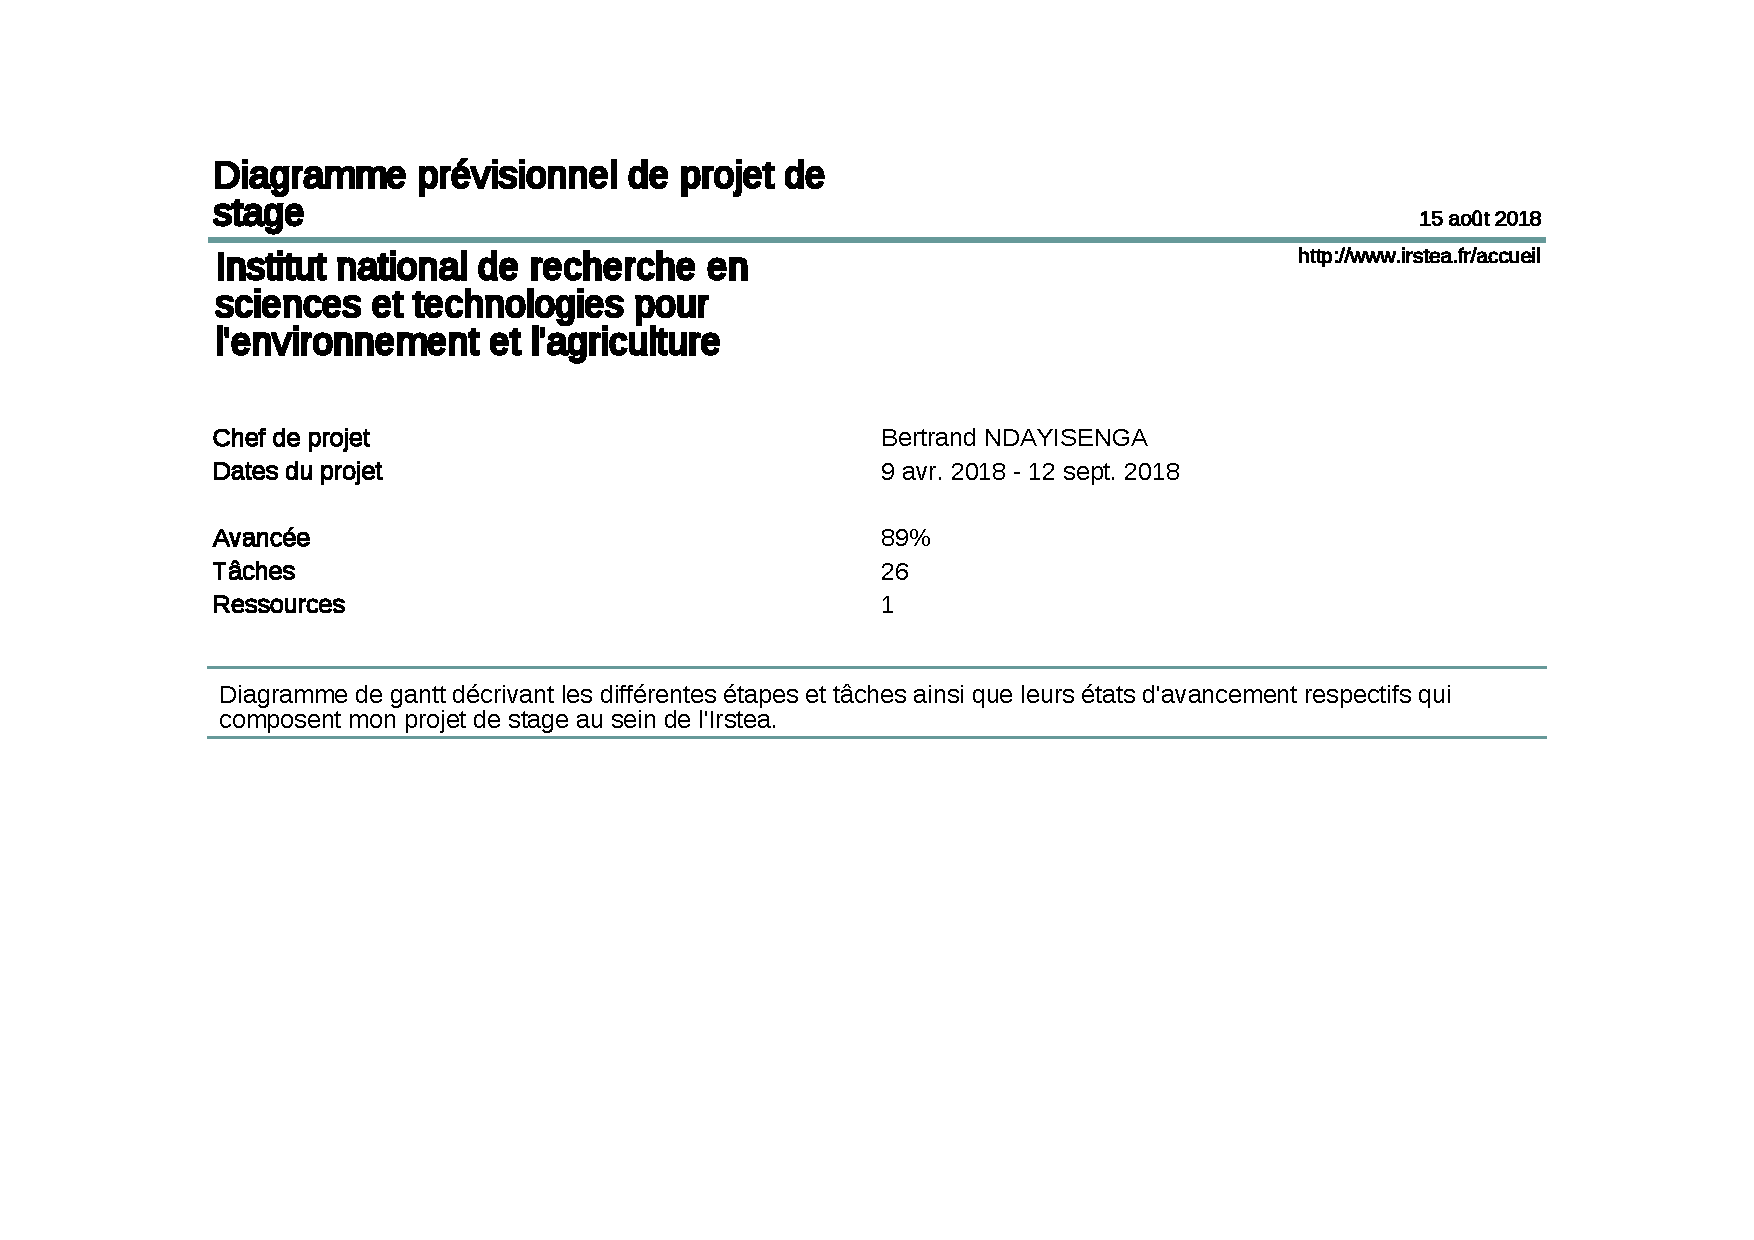
\includepdf[pages={1,2,5}]{pdfFiles/GantPrevisonnel.pdf}
    \renewcommand{\partname}{}
\renewcommand{\chaptername}{}
\renewcommand{\thechapter}{}
\renewcommand{\thesection}{}

\part{Projet OPEROSE}
\section{Présentation du projet OPEROSE}
L’équipe COPAIN participe à l’organisation opérationnelle du Challenge \gls{ANR} \gls{ROSE}. Ce dernier, a pour objectif d’encourager le développement de solutions innovantes autonomes en matières de désherbages intra-rang de grandes cultures à fort écartement (ex maïs, tournesol, …) et des cultures légumières de plein champ afin de réduire l’usage des herbicides. En effet, des solutions technologiques existent pour éliminer les mauvaises herbes entre deux rangs de cultures(l’inter-rang) sans utiliser des produits chimiques, mais peu d’alternatives sont proposées pour le désherbage de l’intra-rang, c’est-à-dire entre les plants d’un même rang. C’est ainsi que le ministère chargé de l’Agriculture et de la Transition Écologique en partenariat avec le ministère de la Recherché et l’ANR, dans le cadre du plan Ecophyto II, ont lancé le challenge ROSE.  Ce Challenge a débuté en janvier 2018 et durera quatre ans, durant lesquelles, quatre campagnes d’évaluations seront menées par le consortium en charge de l’organisation à savoir IRSTEA/LNE avec la participation de VetAgro Sup.  

L’avancée des travaux sera mesurée tout au long du projet lors de rencontres annuelles sur le terrain durant lesquelles les chercheurs réaliseront certaines tâches précises, dans un cadre de répétabilité et de reproductibilité des expériences menées. Les confrontations seront organisées selon une procédure élaborée en concertation avec les chercheurs, par le LNE/IRSTEA. 

\begin {figure}[!h]
\begin{center}

    \hbox{ 
    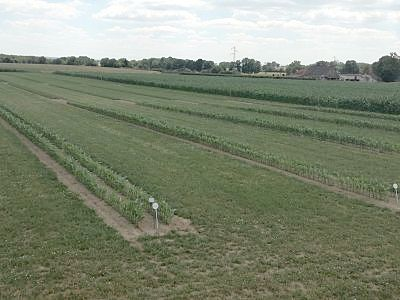
\includegraphics[width=5cm]{images/imageRang1.jpg}
    \hspace*{1cm}  %% pour mettre un espace %(horizontal) de 5cm entre les deux images
    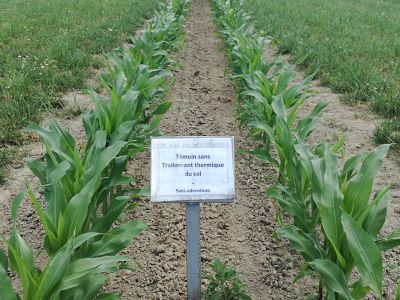
\includegraphics[width=5cm]{images/imageRang2.jpg}
  }
\caption{Rangées de cultures pour le challenge Rose}
\label{Rangées de cultures pour le challenge Rose}
\end{center}
\end {figure}
\textbf{site web du challenge ROSE : }\url{http://challenge-rose.fr/}



\section{Ma mission au sein du projet}
Ma mission au sein du projet fut donc de contribuer au développement d’une solution de collecte et stockage de données acquises sur les parcelles agricoles mises à la disposition des participant au challenge. 

Plus précisément, il s’agissait de concevoir, modéliser et implémenter une base de données qui servira à stocker les données collectées au moyen de capteurs implantés sur le site de Montoldre. Cette base de données pourra participer à un dispositif d’aide à la décision permettant aux participants du challenge de savoir à quel moment intervenir sur les parcelles et ainsi mettre en pratique leurs solutions de désherbage.  

L’un des points importants à cette mission était de rendre cette base de données assez générique pour pouvoir être alimenter par différents types de données provenant de différents types de capteurs. 

En parallèle à cette tâche, je devais également proposer une solution d’extraction, transformation de données capteurs météo déjà implantés. En effet, deux stations météo, ont été installé sur le site de Montoldre. Tout l’enjeu de cet exercice était de pouvoir automatiser, par le biais d’un petit programme, les tâches d’extraction et de transformation. Les données sont ainsi relevées sous leurs formats d’origine convertit dans des formats standard avant d’être sauvegarder dans la base de données. 

Finalement, après avoir fait la base de données capteurs, et le petit programme extracto-chargeur, il fallait penser à la meilleure façon de d’envoyer toutes ces données au LNE qui s’occupe de la mise à disposition de ses données. 

 
\subsection{Cahier de Charge}
 \begin{itemize}
      \item Modéliser une base de données générique pouvant stocker n’importe quel type de données capteurs. 
     \item Extraire, transformer et stocker les données des capteurs météo déjà présentes sur le site de Montoldre.
     \item Automatiser la tâche précédente et la rendre disponible sur différents système d’exploitation 
     \item Proposer une solution pour un envoie régulier et à distance de données différents données météo. 
     \item Produire une documentation assez précise pour des futurs utilisateurs. 
     \item Mettre à disposition un outil interne de visualisation de des données. 
 \end{itemize}

\subsection{Analyse de l’existant} 
Étant arrivé presque en début de projet, il est évident que la plupart des tâches venaient juste d’être reparties. Cela m’a permis de m’approprier très rapidement le projet, ce qui m’a permis de le comprendre dans sa globalité et plus particulièrement mon sujet de stage.   

Quand j’ai commencé à travailler sur le projet OPEROSE, une étude sur le recensement des caractéristique capteurs avait déjà été mené en amont par des d’autres stagiaires et des permanents de l’IRSTEA. 

\subsection{Choix des outils et technologies}

Conscient que le projet OPEROSE réunissait plusieurs acteurs de différents domaines répartis sur toute la durée du projet, le choix des technologies et outils utilisés se devait de suivre quelques critères pour permettre une bonne maintenabilité future. Voici quelques critères qui ont influencé nos choix : 
\begin{itemize}
 

  \item la technologie ou l’outil utilisé doit être choisi en équipe : en effet durant mon stage la technologie a utilisé n’était pas imposé. Je n’ai pas non plus voulu une technologie qui m’était plus familière ou dont j’avais plus l’habitude. Je me suis plus orienté vers la technologie qui sont déjà utilisé ou si non, je demandais quelle technologie conviendrait le mieux et on arrivait à trouver un consensus. Cela est valable par exemple pour le choix du langage de programmation utilisé. 

  \item Les logiciels utilisés, pour des raison pratique, se devaient d’être libre d’utilisation et gratuit. 

   \item facile à utiliser : outils dont l’utilisation est intuitive pour réduire au maximum le temps d’apprentissage 
\end{itemize}
Ces critères on fait que je choisisse un outil par rapport à un autre, une technologie par rapport à une autre, même si tous les critères n’était pas rempli tout le temps. Cela m’a permis de me fixer un cadre de ne pas me perdre dans l’immense panoplie d’outils proposé mais surtout de me dépasser en s’adaptant aux nouveaux outils qui ne m'était pas familière. 

L'image \ref{fig : Outils et Technologies utilisés}résume l’ensemble des outils et technologie utilisés 
\begin{figure}
\begin{center}
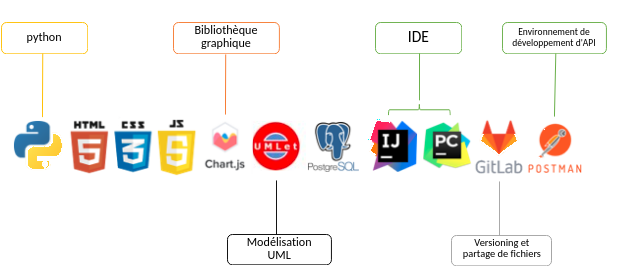
\includegraphics[width=400px]{images/logicielutilises.png}
\end{center}
\caption{Outils et Technologies utilisés}
\label{fig : Outils et Technologies utilisés}
\end{figure}

\section{Mise en œuvre de la solution} 

La base de données étant un élément essentiel du projet, elle se devait d’être très générique. En effet, cette contrainte fait partie du cahier des charges. Elle doit pouvoir accueillir les données des capteurs déjà existants mais aussi des capteurs qui pourraient être ajoutés plus tard. Cette base doit pouvoir sauvegarder aussi bien les données des capteurs que leurs caractéristiques et les métadonnées.

Malgré l'importance de la modélisation de la base de données nous avons pris la décision de commencer par l'extraction des données des stations météo. Cela m'a permis de me familiariser avec les données issues des capteurs. Sur les conseils de mon maître de stage, j'ai réalisé un modèle de base de données assez simple et le plus évolutif possible, facile à comprendre, pour avoir une idée générale et on s’est réservé le droit de le modifier et de l’améliorer tant que cela soit possible. 

Simultanément, j’ai pu commencer à travailler sur le programme extracto-chargeur de données météo des stations se trouvant sur le site de Montoldre. Ainsi j’ai pu appréhender la notion de données sur les données en générale et les données météo en particuliers.  

 
Sur le site de Montoldre, deux stations météo avaient été installées. Valentin Mère, stagiaire sur le même projet basé sur le site de Montoldre s’était occupé de la partie acquisition de données comme par exemple installer et tester le bon fonctionnement des stations. Depuis le site d’IRSTEA Aubière, j‘avais accès aux données via le réseau Intranet d’IRSTEA. Une visite sur les lieux m’a permis de me rendre compte des dispositifs avec lesquelles je travaillais à distance.  

\subsection{Les stations météo du site de Montoldre} 

\subsubsection{Station météo Sencrop}

\begin{wrapfigure}{r}{.3\textwidth}
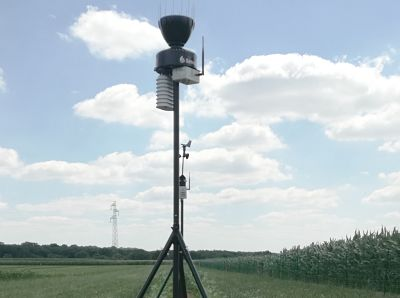
\includegraphics[width=4cm]{images/imageRang3.jpg}
\end{wrapfigure}
Sencrop est un ensemble de deux stations, un pluviomètre(raincrop) et un annémomètre (windcrop) produit par une société française basée à Lille et spécialisée dans la météo pour l’agriculture. La station Sencrop est dotée de capteurs qui enregistrent la pluviométrie, la température de l’air, l’hygrométrie, la vitesse et la direction du vent. Elle envoie ses données toutes les quinze minutes via une API et celles-ci peuvent être accessibles sur un smart phone, une tablette ou un ordinateur. Cette station a été installée au courant du mois de juin 2018. 

\subsubsection{Station météo Davis vantage Pro 2}

Installée en 2010, la station Davis est un produit du groupe CIMA TECHNOLOGIE FRANCE. Station sans fil, elle comprend une suite intégrée de capteurs météo et une console de visualisation des données, mesure. Elle mesure le vent (vitesse et direction), la pluviométrie, la température et l'humidité sous abri à ventilation naturelle, l'humidité intérieure et extérieure, pression barométrique. La portée radio en espace libre est de 300 m.



\section{Les diagrammes de séquences}
 
Les diagrammes ci-dessous décrivent les séquences d’extraction des données à partir des stations météo sencrop et davis vantage pro 2 ansi que leurs chargment dans des bases de données intermédiaire.

\subsection{Séquence pour la station sencrop.}
Sencrop met à disposition de ses clients, détenteurs d’une de leurs stations, une plateforme de visualisation des relevés. Cette plateforme présente des données en générale de façons agrégés mais permettant d’avoir une bonne lecture de la situation météorologique selon une plage de temps que l’on souhaite. Elle met également à disposition une API, qui par des requêtes bien précises, permet d’avoir les relevés brutes.  

Il faut donc a avoir un compte sencrop et se connecter à l’ \gls{API}. une fois la connexion établit, un jeton ayant une date d’expiration est généré, et l’on peut faire ainsi une requête. Ce processus peut donc être automatiser via un script python et être exécuté régulièrement via un gestionnaire de tâches. La grande difficulté réside dans le fait de bien comprendre en amont, la structure des requête c’est-à-dire le nombre et le type de paramètres qu’il faut envoyer mais aussi la structure des données que l’on reçoit. C’est pour cela que sencrop a prévu une documentation pour pouvoir utiliser l’API. 
\newline
\url{https://developer.sencrop.com/guide/}  
\begin{figure}[!h]
    \label{diagramme de séquence stéation sencrop}
    \centering
     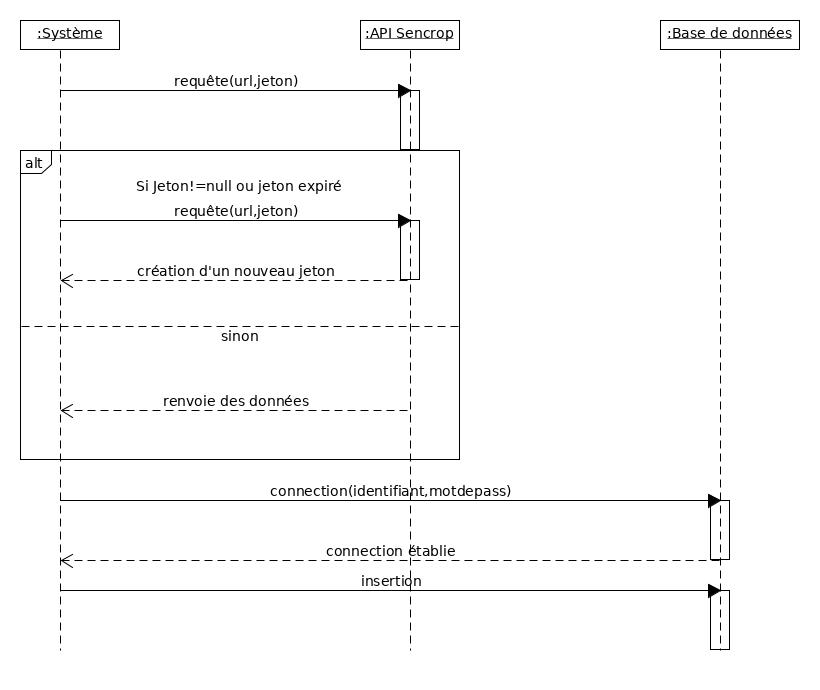
\includegraphics[width=.7\textwidth]{images/sencrop_senquence_diagrame.jpg}
    \caption{diagramme de séquence pour l'extraction et le chargement des données de la station sencrop}
  
\end{figure}

\subsection{Séquence pour la station davis vantage pro 2} 
La station météo davis vantage pro 2 génère des fichiers au format .wlk. Ces fichiers sont modifiés quotidiennement et ne contienent que les données du mois courant. Ainsi par exemple pour le mois d’août 2018 un fichier de nom 2018\_08.wlk sera généré. Celui-ci sera modifié quotidiennement pour contenir tous le données à partir du 01 jusqu’au jour précédent. Un logiciel, fourni par l’entreprise propriétaire, pour décoder les fichiers .wlk existe mais il n’est pas gratuit.Plus encore, il n’est pas pas multiplateforme et l’utilisation de celui-ci en ligne de commande pour automatiser les tâches est quasi-impossible car il nécessité plusieurs paramétrés. Nous nous sommes donc tournés vers des outils libres qui existeraient sur internet pour décoder les fichiers wlk.J'ai ainsi trouvé un utilitaire permettaant non seulement de décoder les fichiers .wlk mais aussi de générer des fichiers au format sql pour alimenter une base de données. Ceci nous a beaucoup aidé car il ne restait plus que la tâche d'automatisation  de décodage des fichiers .wlk et celui de l’insertion. Mais il s’est avéré qu' à certains endroits, l’utilitaire produsait des erreurs de sorti. La grande difficulté fut de pouvoir personnalisé les sortis attendues pour qu’elles correspondent aux résultats escomptés. 

\begin{figure}
    
    \centering
     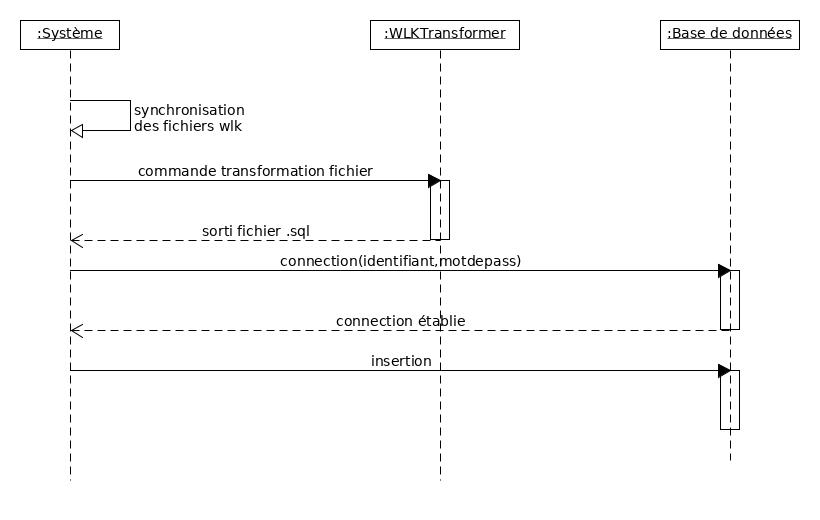
\includegraphics[width=.7\textwidth]{images/davis_senquence_diagrame.jpg}
     \caption{ Séquence pour l'extraction et le chargement des données de la station Davis vantage pro2}
     \label{diagramme de séquence station sencrop}
\end{figure}


\begin{figure}[!h]
    \centering
     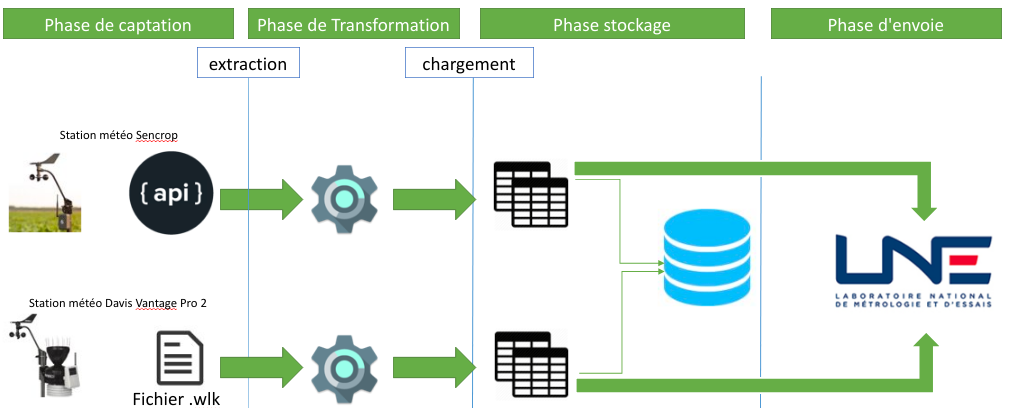
\includegraphics[width=1\textwidth]{images/processusOperose.png}
     \caption{ Séquence d'extraction de chargement et d'envoie données pour le projet OPEROSE}
     \label{diagremme de séquence station Davis}
\end{figure}
     


\section{modélisation de la base de données}
la modélisation de la base de données s'est fait progressivement tout au long du stage. Chaque fois on essayait de l'améliorer en y apportant les ajouts nécessaire pour la faire correspondre à l'idée de départ, d'une base de données générique. Au moment de la rédaction du rapport, sa modélisation n'est pas encore fini ou plutôt n'est pas encore validé. Toute fois, nous avons décidé d'y insérer des données et la testée jusqu'à ce qu'à ce que nous rencontrions un problème.
\subsection{Principe d'une base de données générique}
D'une manière générale, lorsqu'on modélise une base de données, on regroupe entre eux les objets ayant les mêmes propriétés dans entités. Par exemple pour une base de données qui stocke des objets de type moutons et voitures, on aura des entités(tables) moutons et voiture comme dans l'exemple qui suit : 

\begin{figure}[h!]
\begin{center}
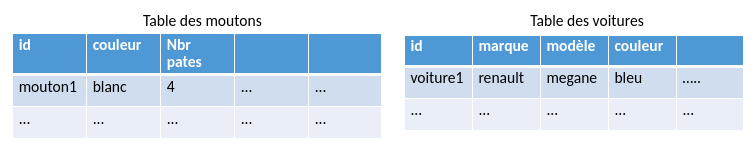
\includegraphics[width=1\textwidth]{images/bd_image1.png}
\end{center}
\caption{exemples de tables d'une base de données}
\label{exemples de tables d'une base de données}
\end{figure}

la modélisation devient d'autant plus difficile si dès le départ on ne connaît pas l'ensemble des objets que l'on doit stocker. En d'autres mots, on souhaite faire une base de données pour contenir plusieurs type d'objets dont les propriétés ne sont pas connu à l'avance. Dans l'exemple ci-dessus, ça correspondrait à stoker, en plus des moutons et des voitures, des immeubles, des personnes et tout autre type d'objet. Pour y remédier, on fait intervenir les bases de données générique. Cela consiste modifier la structure de notre entité et la faire correspondre à une système proche du schéma (clé:valeur). Ce cas de figure fait passer les propriétés des entités dans les colonnes.
l'exemple ci-dessous illustre bien ces propos

\begin{figure}[h!]
    \begin{center}
    \label{exemple de table d'une base de données générique}
         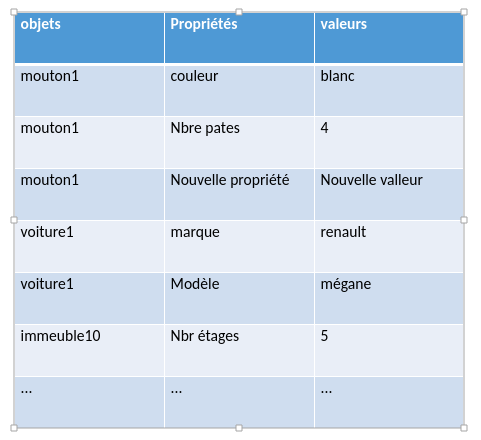
\includegraphics[width=0.4\textwidth]{images/bd_image2.png}
    \caption{exemple de table d'une base de données générique}
    \end{center}
\end{figure}


\subsubsection{Modélisation}
La valeur d'une donnée en générale et d'une donnée capteur émanant d'une mesure en particulier est d'autant plus important que celle-ci fait apparaître la dimension espace et la dimension temps.
A quoi nous servirait par exemple d'avoir 30$^\circ$ celsius, si on ne se pas à quel endroit fait référence à cette mesure ni à quelle moment elle a été relevé. Ce principe nous a guidé dans la modélisation de la base de données.

Pour faire intervenir la dimension espace, on s'est dit qu'un capteur est localisé dans un noeud et un noeud est un point d'un réseau de capteur. Ainsi chaque relevé peut être localisé avec un certain degré de précision.
La dimension temps sera matérialisée par le fait que chaque relevé sera identifiée par un attribut date. 
\begin{figure}[!h]
    \begin{center}
         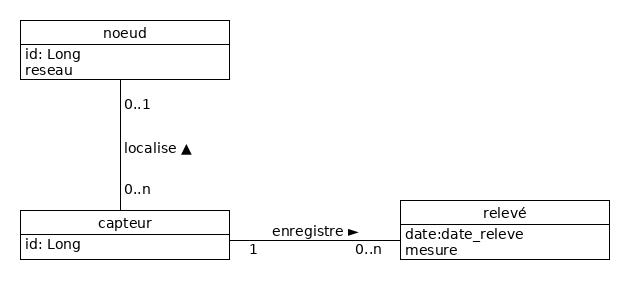
\includegraphics[width=1\textwidth]{images/uml_image1.jpg}
    \caption{modélisation UML phase 1}
    \label{fig:modélisation UML phase 1}
    \end{center}
\end{figure}

Ne connaissant pas à l'avance quel types de capteurs on aura ni les caractéristiques de ses derniers, il nous est impossible de modéliser la table capteurs. Mais en appliquant le principe de générécité cité ci-haut, on peut alors extraire les caractéristique liés au capteurs pour les mettre dans un autre table. On appliquera le même principe pour les noeuds.
\begin{figure}[!h]
   \begin{center}
        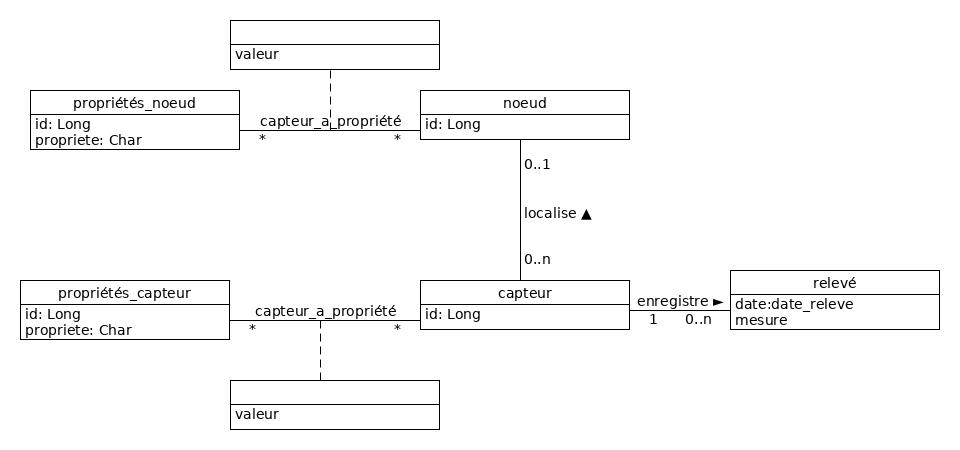
\includegraphics[width=1\textwidth]{images/uml_image2.jpg}
    \caption{modélisation UML phase 2}
    \label{fig:modélisation UML phase 2}
   \end{center}
\end{figure}
En continuant à raisonner de façon générique, on arrive à modéliser notre base de données comme sur la figure \ref{ Base de données OPEROSE}. Si l'on regarde plus attentivement, on se rend compte qu'une table, de la base de données contiendra beaucoup plus de données que les autres. Dans notre cas il s'agit de la table \textbf{releve} qui stockera toutes les mesures de tous les capteurs. Le fait de transposer les données d'une table normale à une table générique augmente considérable le nombre d'enregistrements. Cela a des conséquence sur l'espace à allouer à la base de données mais aussi sur la complexité en temps d'exécution des requêtes. Une des solutions pour pallier à ce problème peut être d'utiliser les vues matérialisés pour certaines requêtes.


% image de la base de données
\begin{landscape}
\begin{figure}
   \begin{center}
       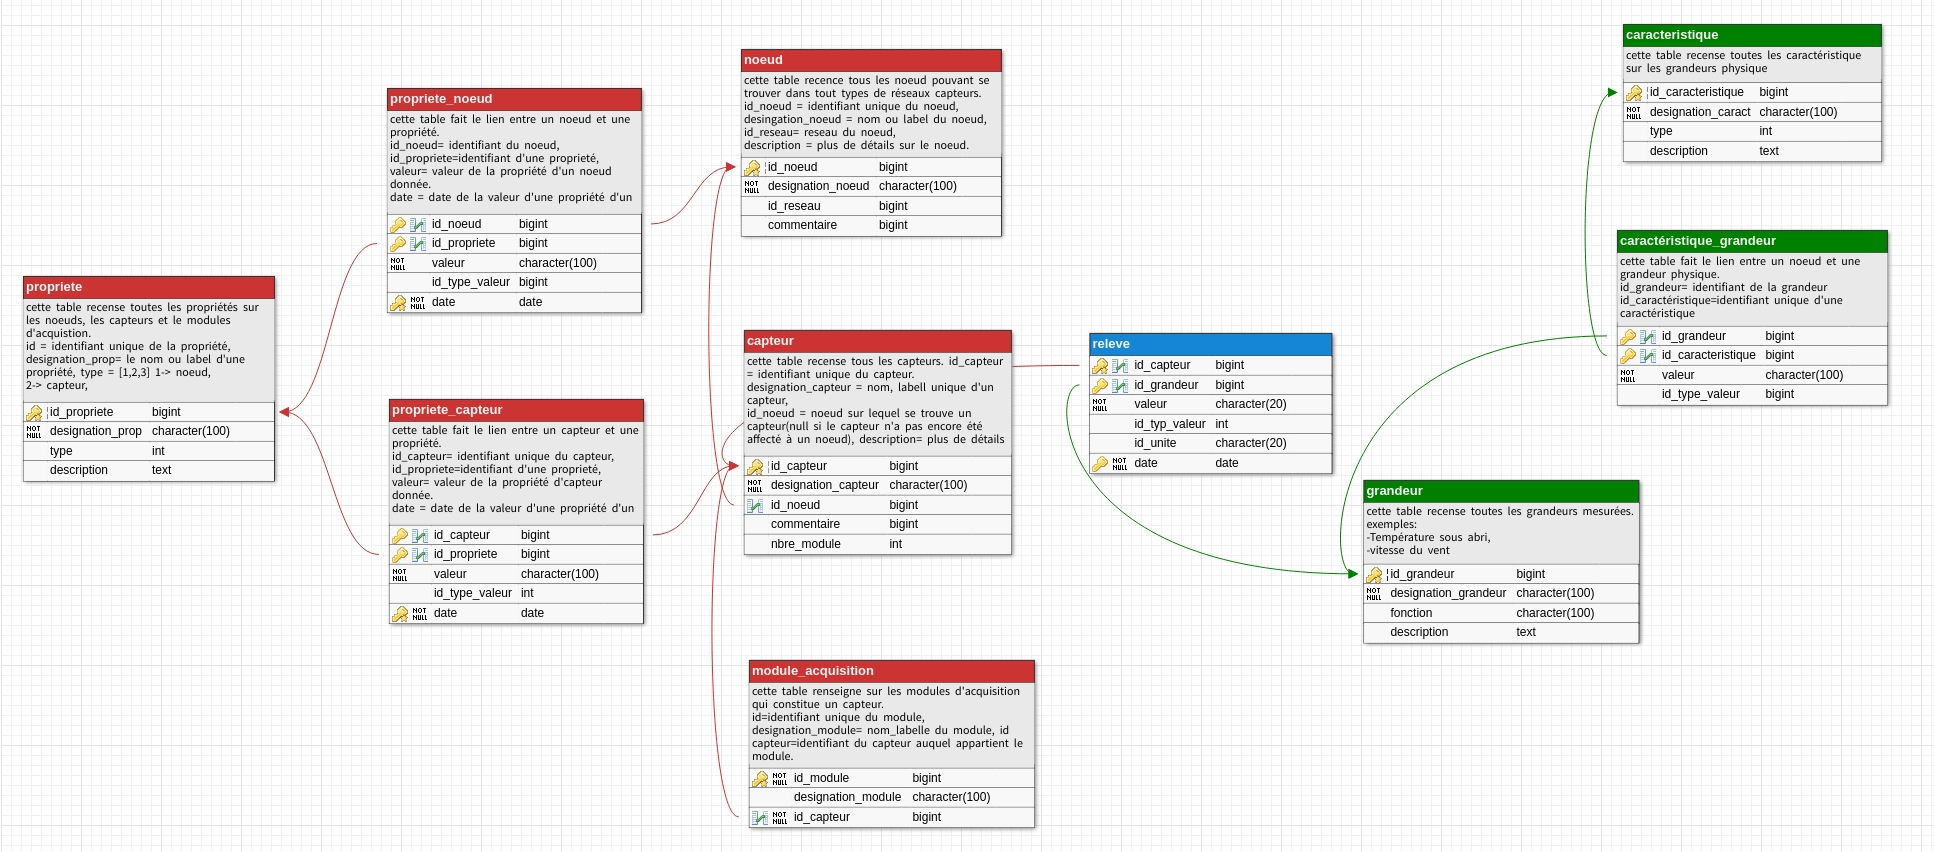
\includegraphics[width=1.8\textwidth]{images/bd_image3.jpg}
    \caption{ Base de données OPEROSE}
     \label{ Base de données OPEROSE}
   \end{center}
\end{figure}
\end{landscape}







\section{Visualisation des données}
Une page de visualisation des données a été crée en utilisaant les langanges HTML, CSS, PHP, JavaScript et une librairie permettant la création de graphique. Sur cette page on retrouve par exemple tous les informations concernant un noeud, tous les informations sur les capteurs d'un noeud données ainsi que les données des capteurs localisés sur un noeud données représentés sous forme de graphiques comme dans comme dans la figure.
Une des amélioration a apporté à la visualisation, serait de pouvoir croiser les données pour pourvoir permettre une comparaison rapide des relevés capteurs. En effet, pour l'instant, pour une même données \begin{math}x \end{math} (exemple : température de l'aire) mesurée par deux capteurs distincts \begin{math}C_{1}\end{math} et \begin{math}C_{2}\end{math}, on a deux graphiques distincts, ces derniers étant construit par capteurs. Le but serait donc de combiner les 2 graphiques en un seul graphique ce qui permettrait une comparaison plus rapide
\begin{figure}
    \centering
    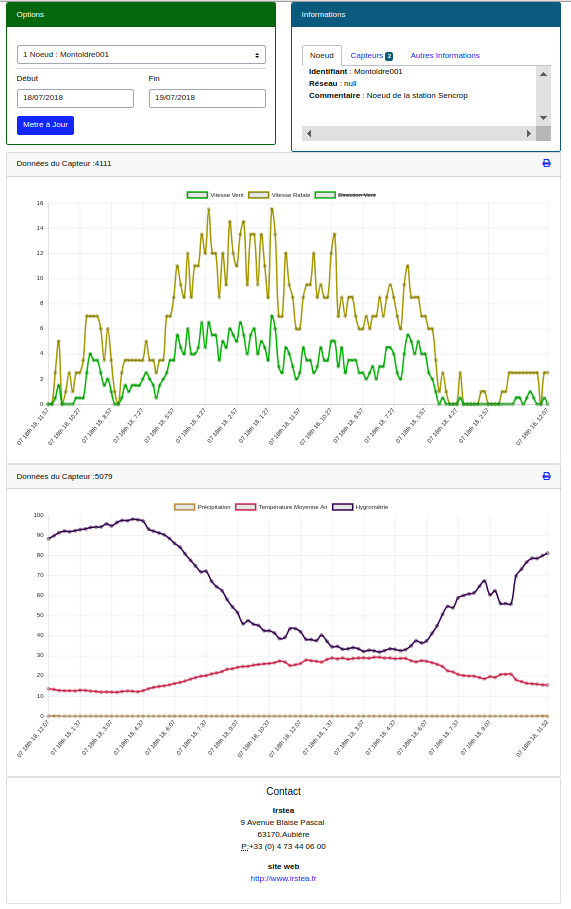
\includegraphics[height=1\textheight]{images/db_visualisation.png}
    \caption{page de visualisation des données}
    \label{fig:page de visualisation des données}
\end{figure}



    \renewcommand{\partname}{}
\renewcommand{\chaptername}{}
\renewcommand{\thechapter}{}
\renewcommand{\thesection}{}

\part{projet MULTIPASS}
\section{Présentation du projet} 
L'agriculture numérique, fait que les exploitations agro-pastorales sont aujourd’hui une source immense de données. De ce fait, les institutions techniques agricoles ont formulé dix recommandations pour faciliter l’accès et et la valorisation de ces données. Ainsi ,à travers son financement au moyen du compte spéciale \"développement agricole et rural\" (CASDAR), le ministère en charge de l’agriculture lance en 2007 le projet  MULTIPASS. Ce dernier vise faire émerger de nouveaux services pour l’agriculteur dans une chaine de confiance gérant les consentements d’accès aux données des exploitations. Le projet renforcera ainsi la confiance nécessaire au partage de données et permettra d’apporte une solution aux questions des agriculteurs sur la maîtrise de leurs données et la transparence des usages qui en sont faits. 

Plus précisément, les objectifs du projet sont les suivants : 

\begin{itemize}
    \item Proposer un écosystème de gestion des consentements interopérable entre les acteurs qui apporte confiance, simplification et sécurité aux producteurs et valorisateurs de données. 
    \item Favoriser l’innovation ouverte, c’est\-à\-dire l’émergence d’applications agronomiques couplées aux données des agriculteurs provenant de n’importe quelle source de données ou objet connecté, pour éviter le risque de concentration de l’innovation. 
    \item Favoriser la création de connaissances par l’analyse de données massives d’exploitations, dans une chaîne de confiance. 
\end{itemize}

Partenaires : ARVALIS (Coordinateur), ACTA, FIEA, IDELE, Irstea, Orange, Smag.

Financement : \gls{CASDAR} Recherche Technologique 
 \section{Ma mission au sein du projet} 

Ma mission au sein du projet MULTIPASS était de mener une étude sur les différentes techniques d’anonymisation des données. Cette étude pouvait se décliner sur deux plans : premièrement faire un état de l’art sur les techniques d’anonymisation déjà existantes et proposer une façon de les appliqués au domaine agricoles et deuxièmement faire des tests sur des jeux de données. Dans cette  partie du rapport, j'ai identifié quelques techniques parmi les plus utilisées sur l’anonymisation des données : leurs points forts ainsi que leurs faiblesses. 
\renewcommand{\partname}{}
\renewcommand{\chaptername}{}
\renewcommand{\thechapter}{}
\renewcommand{\thesection}{}

\chapter{Anonymisation des données}
\subsection{Qu'est-ce que l’anonymisation?} 

l’avis du G29\footnote{Groupe de travail institué par l’article 29 de la directive 95/46/CE. Il s’agit d’un organe consultatif européen indépendant
sur la protection des données et de la vie privée. Ses missions sont définies à l’article 30 de la directive 95/46/CE et à l’article
15 de la directive 2002/58/CE.}[4] rappelle que \textbf{\emph{l’anonymisation}}, au sens de la directive 95/46/CE (abrogé par le règlement numéro 2016/679 dit \gls{RGPD})
\begin{em}
    "est le résultat du traitement des données personnelles afin d’empêcher de façon irréversible, toute identification"
\end{em}  

L’anonymisation est donc ce processus qui supprime tout lien directe ou indirecte entre une personne et la donnée qui la concerne. Mais le défi majeur de l’anonymisation réside dans le fait de pouvoir garder l’utilité de l’information que contient une donnée.  En effet, plus on cherche à anonymiser plus grande est la perte de l’information.  
Ainsi donc, l’anonymisation et la re-identification ont fait et font toujours l’objet de plusieurs études. Certains cherchent des techniques de plus en plus performantes pour rendre anonyme, d’autres, des techniques pour casser les techniques précédentes. Nous citerons l'exemple de Lantanya Sweeney, qui, au début des années 2000, prouva qu’une méthode (appelé aujourd’hui pseudonymisation) n’était pas efficace pour anonymiser et   proposa une autre méthode nommée k-Anonymat, ([5], que nous verrons plus tard. 

\subsection{Différence entre l’anonymisation et la pseudonymisation}

Le caractère irréversible doit être établie pour dire qu’il y a anonymisation. Dans le cas contraire il s’agit d’une pseudonymisation. Nombreux sont ceux qui confondent l’anonymisation et la pseudonymisation. Ce dernier, se dit d’un processus qui remplace un attribut (généralement un attribut unique) par un autre (appelé pseudonyme) dans un enregistrement [6, p. 29]. 

L’avantage de la pseudonymisation est que tant qu’on ne traite pas les champs identifiants, les résultats sur les autres champs sont identiques que des résultats effectués sur une base non anonymisée. Toutefois, la pseudonymisation reste fragile aux attaques de type record linkage, mis en évidence par Latanya Sweeney. Elle put identifier une partie des individus issus d’une base de données médicale (pseudonymisée) croisée avec une liste électorale publique. 

\subsection{Pourquoi faut-il anonymiser?} 

L’objectif principale de l’anonymisation est de réduire à un niveau acceptable le risque de réidentification. Il faut anonymiser car, des règles de confidentialité et de sécurité sont imposés par la loi surtout quand il s’agit de données personnelles. Ces lois sont là pour empêcher des tierces personnes à accéder à des données personnelles [7]. 


\subsection{Quand faut-il anonymiser?} 

S’il est évident qu’il est nécessaire d’anonymiser dès lors que des données (à caractères personnels) quittent un environnement sécurisé pour être rendus publique, il convient aussi d’anonymiser les données dès leur processus de réception. Ce deuxième cas, suppose que le risque zéro n’existe pas et, qu’aussi sécurisé soit-elle, une base de données peut toujours tomber aux mains d’une personne malveillante. 

Ainsi on distingue deux stades pour l’anonymisation: 

L’anonymisation à bref délai: les données collectées sont tout de suite anonymisées (dans un délai allant de quelques secondes à quelques minutes). Le responsable de traitement à l’obligation d’indiquer son identité et la finalité du traitement pour la courte période pendant laquelle les données ne sont pas anonymisées.  

L’anonymisation ultérieur: le processus d’anonymisation se fait une fois le délai de conservation des données dépassé. On choisit alors de ne pas supprimer les données et de les conserver à des fins de statiques par exemple. Les données devront être collectées et traitées dans le strict respect de la Loi de 1978. 

[8] 

\subsection{Comment anonymiser?} 

Le processus général pour anonymiser un ensemble de données est de supprimer tous les attributs identifiant (ex: nom, le numéro de sécurité sociale, etc.), et ensuite de modifier les attributs quasi-identifiants (âge, adresse, etc.).  

Parmi les techniques pour l’anonymisation des données on distingue deux grandes familles:  

Les techniques de généralisation: techniques qui consistent à généraliser ou diluer les données personnelles de façon à ce qu’elles perdent en précision et qu’elles ne soient plus spécifiques à une personne mais communes à un ensemble de personnes. 

Les techniques de randomisation:  techniques d’anonymisation qui altèrent la véracité des données dans le but de supprimer le lien fort entre les données et la personne [7]. 

\subsection{Critères d’évaluation des techniques d’anonymisation}

Selon l’état actuelle des technologies, trois risques essentiels sont à tenir compte dans le processus d’anonymisation:  

\begin{itemize}
 
    \item \textbf{L’individualisation}: risque de pouvoir isoler une partie ou l’ensemble des enregistrements d’un individu dans un jeu de données. C’est-à-dire que dans un jeu de données si on arrive à identifier toutes ou une partie des enregistrements (ligne) correspondant à un individu, alors, le jeu de données peut être individualisé. 

    \item \textbf{La corrélation:} risque de pouvoir relier deux enregistrements correspondant à un même individu. Les enregistrements peuvent appartenir à un seul jeu de données ou à des jeux de données distincts. C’est-à-dire que dans un jeu de données si on arrive à prouver qu’au moins deux enregistrements (lignes) correspondent à un seul et même individu ou groupe d’individu, alors il est possible de corréler. Toutefois, il est possible d’avoir une technique qui ne résiste pas à la corrélation mais qui résiste à la l’individualisation.  

    \item \textbf{L’inférence:} risque de pouvoir déduire, avec une probabilité élevée, la valeur d’un attribut à partir d’un ou d’un ensemble d’autres attributs. Pour comprendre ce risque on peut prendre l’exemple suivant: il est facile de déduire le salaire (même s’il est anonyme) d’un individu rien qu’en ayant connaissance des attributs poste et ancienneté [10]. 
\end{itemize}
\chapter{Techniques d'anonymisation}
%ajouter les grandes familles des technique
\section{les Techniques de généralisation}
\subsection{K-anonymat} 

Le K-anonymisation est une technique d’anonymisation qui empêche qu’une personne ne soit isolée dans un jeu de données. Elle permet ainsi de regrouper un individu avec au moins K autres individus, de sorte qu’il y ait moins de chance de retrouver l’individu en question. En d’autres mots, on généralise certains attributs de telle manière à ce que ces derniers soient identiques pour un groupe de K individus [4;11]. 

\paragraph{Etapes de la k-anonymisation:} 
\begin{itemize}
    \item  Déterminer les ensembles d’attributs qui peuvent être utilisés pour croiser les données anonymes avec des données identifiants. 

    \item Réduire le niveau de détail des données de telle sorte qu’il y ait au moins k individus qui ont la même valeur de quasi-identifiants. 
\end{itemize}

%% ajout d'exemple
\begin{figure}[!h]
    \centering
    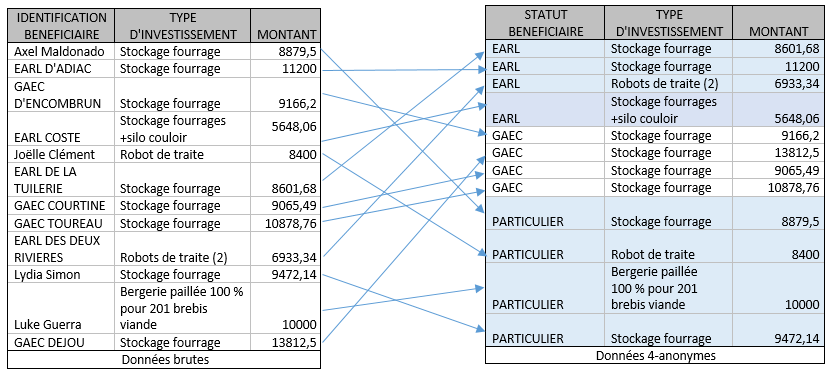
\includegraphics[width=1\textwidth]{images/anonymisation/k_anonym_image1.png}
    \caption{Exemple d'une k-anonymisation : données 4-anonymes}
    \label{Exemple d'une k-anonymisation : données 4-anonymes}
\end{figure}


\paragraph{Evaluation du k-anonymat:}  
\begin{itemize}
    \item \textbf{Individualisation :} étant données les classes d’équivalence, nous savons qu’au moins k individus partagent certains attributs dans le jeu de données. Il ne devrait plus être possible d’isoler un individu dans un groupe de k autres individus. 

    \item \textbf{Corrélation:} il est possible de relier les enregistrements par groupe de k-individus. Au sein d’un même groupe, la probabilité que deux enregistrements correspondent à un individu est de 1/k. 

    \item \textbf{Inférence:} si tous les k individus d’une classe d’équivalence ont la même valeur pour un attribut donné et que cette information est sensible, il suffit de connaître à quelle classe d’équivalence appartient un individu pour déduire sa données sensible. 
\end{itemize}
 
Alors que k-anonymat protège contre la divulgation d'identité, il n'offre pas une protection suffisante contre la divulgation d'attributs. Cela a été reconnu par plusieurs auteurs[13], [14]. Deux attaques ont été identifiées dans: attaque d'homogénéité et l'attaque de connaissances de fond[14]. 
\subsection{L-diversité}
%ajout d'exeple

La l-diversité est une technique d’agrégation qui étend la k-anonymisation. En effet, il est toujours possible de déduire les informations sensibles si les k individus d’une classe d’équivalence possèdent tous la même information sensible Figure \ref{fig:Données 3-anonymes mais pas l-diverses}

La l-diversité ajoute une contrainte selon laquelle les k-enregistrements d’une classe d’équivalence doivent avoir au minimum l valeurs distinctes comme dans la figure \ref{fig:Données 3-anonymes et 3-diverses}

%ajout d'exemple

Dans l’exemple \ref{fig:Données 3-anonymes mais pas l-diverses}, si l’on sait qu’une personne cultive une grande culture (blé, mais, orge) on déduit quel type de pesticides elle utilise, dans notre cas, les fongicides (\textbf{\textbf{homogeneity Attack}}).  Comme citer en haut, l’inférence est la grande faiblesse du k-anonymat.La l-diversité vient y remédier en y ajout une contrainte Figure \ref{fig:Données 3-anonymes et 3-diverses}. 

Ainsi donc on n’est plus en mesure de deviner le type de pesticides utilisé en fonction du type de culture.  

Cependant, avec une attaque d’inférence probabiliste, on peut par exemple déduire avec une certaine probabilité assez élevée, le type de pesticide utilisé. En effet, si la personne malveillante sait qu’Alan, qui est la seule personne à avoir une parcelle de 38ha, alors, il lui est possible de deviner, avec une probabilité de 1/3, le type de pesticide qu’Alan utilise (\textit{\textbf{Background Knowledge Attack}}). \cite{nguyen_techniques_2014}
\begin{figure}[!h]
    \centering
      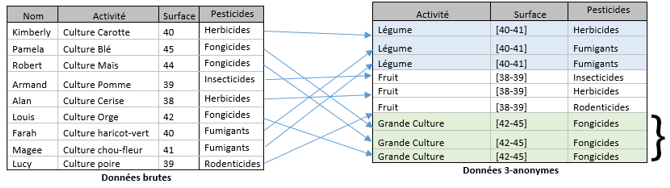
\includegraphics[width=1\textwidth]{images/anonymisation/l_divers_image1.png}
    \caption{ Données 3-anonymes mais pas l-diverses}
     \label{fig:Données 3-anonymes mais pas l-diverses}
   
\end{figure}


\begin{figure}[!h]
    \centering
      
   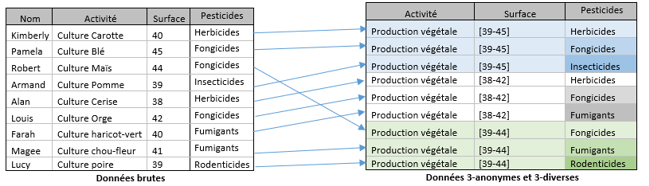
\includegraphics[width=1\textwidth]{images/anonymisation/l_divers_image2.png}
    \caption{Données 3-anonymes et 3-diverses }
     \label{fig:Données 3-anonymes et 3-diverses}
\end{figure}

\paragraph{Évaluation de L-diversité : }
\begin{itemize}
    \item \textbf{Individualisation:} la l-diversité empêche que les enregistrements relatifs à un individu soient isolés dans la base de données 

   \item \textbf{Corrélation:} la l-diversité n’apporte pas d’amélioration par rapport au k-anonymat.  

   \item \textbf{Inférence:} bien qu’il ne soit plus possible de faire des attaques par inférence, il reste cependant possible de mener des attaques par inférence probabiliste. 
\end{itemize}



\subsection{T-proximité}
La t-proximité formalise l’idée de la connaissance globale en exigeant que la distribution d’un attribut sensible soit, pour toute classe d'équivalence, proche de sa distribution dans l’ensemble du jeu de données. 
\section{les Techniques de généralisation}
\subsection{La permutation}
Aussi appelé désalignement, ou shuffling, elle consiste à échanger les positions des données dans un jeu de données. En d’autres mots, c’est-à-dire que les données sont là mais pas à la bonne place. Elle est utile quand il est important de conserver la distribution exacte de chaque attribut dans l’ensemble de données. Si deux ou plusieurs attributs sont liés par une relation logique ou une corrélation statique et sont permutés indépendamment l’un de l’autre, ce lien sera détruit [4]. 

\begin{figure}[!h]
    \centering
     \label{exemple d'une permutation}
    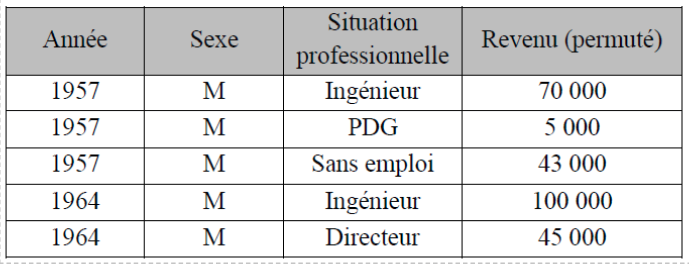
\includegraphics[width=1\textwidth]{images/anonymisation/permutation_image1.png}
    \caption{exemple d'une permutation}
   
\end{figure}
\paragraph{Evaluation de la permutation : }
\begin{itemize}
    \item \textbf{Corrélation:} si la permutation affecte des attributs et des quasi-identifiants, elle peut empêcher de relier «correctement» des attributs entre eux tant à l’intérieur qu’à l’extérieur d’un ensemble de données, mais elle autorise toujours une corrélation «incorrecte» puisqu’une entrée réelle peut se trouver associée à une personne concernée différente. 

    \item \textbf{Inférence:} Des déductions peuvent encore être tirées de l’ensemble des données, en particulier si les attributs sont corrélés entre eux ou ont des relations logiques fortes; toutefois, sans savoir quels attributs ont été permutés, l’attaquant doit envisager la possibilité que son inférence se fonde sur une hypothèse et seule une inférence probabiliste demeure possible. 

Si les attributs sont liés par une forte relation logique, alors la permutation peut être détectée et peut même être inversée. 
\end{itemize}
\subsection{L’ajout de Bruit} 

L’ajout de bruit consiste à rendre moins précis un ensemble de données en ajoutant ou en retirant de l’information sur les enregistrements tout en conservant la distribution générale. Les enregistrements restent identifiables mais sont moins fiables [15]. 

L’ajout de bruit doit normalement être combiné à d’autres techniques d’anonymisation pour être efficace\cite{noauthor_repertoire_2018-1}.  

\paragraph{Évaluation de l’ajout de bruit : }

\begin{itemize}
    \item  \textbf{Individualisation}: l’ajout de bruit n’empêche pas la possibilité d’une isolation. Même si l’enregistrement est moins fiable, il reste possible d’isoler tous les enregistrements concernant un individu. 
    
    \item  \textbf{Corrélation}: il est toujours possible de relier les enregistrements (issu d’un ou de plusieurs jeux de données différents) d’un même individu. 
    
    \item \textbf{Inférence}: le taux de succès avec une attaque par inférence est beaucoup moins élevé. 
\end{itemize}

\paragraph{Erreurs courantes}:   
\begin{itemize}
    \item Ajout de bruit incohérent : si le bruit ne respecte pas la logique des attributs ou si celui-ci est disproportionné, on peut alors imaginer qu'un attaquant puisse identifier le bruit, le filtrer et ainsi recréer un jeu de données. 
    \item supposer que l’ajout de bruit est suffisant : L'ajout de bruit n'est pas une technique qui se suffit. Pour être efficace, elle doit s'utiliser en complément avec d'autres techniques pour rendre difficile la récupération des données.
\end{itemize}


\subsection{La confidentialité différentielle}
%ajouter du texte sur la confidentialité confidentielle
La confidentialité différentielle est l'une des techniques les plus populaire ces dernières années surtout dans la recherche. En effet, contrairement aux autres techniques, elle est la seule à pouvoir fournir des preuves mathématiques sur la possibilité de borner l'information qui peut être appris sur un individus.

\subsubsection{Formalisation}
soit \begin{math}\epsilon\end{math} un réel et\begin{math}A\end{math} une algorithme probabiliste qui prend pour entrée un jeu de données. Soit \begin{math}imgA\end{math} image de \begin{math}A\end{math}. L'algorithme \begin{math}A\end{math} et dit \begin{math}\epsilon\end{math}-différentiellement confidentiel, si, pour tout jeux de données \begin{math}D_{1}\end{math} et \begin{math}D_{2}\end{math} qui diffèretnt d'une seul élément(l'information a propos d'une seule personne) et pour sous ensemlbe \begin{math}S\end{math} de \begin{math}imgA\end{math},

\[
Pr[A(D_{1})\in S] \leq e^{\epsilon} * Pr[A(D_{2})\in S]
\]
où la probabilité est fondés sur l'aléa introduit par l'algorithme. D'après cette définition, la confidentialité différentielle port sur l'algorithme lui-même, et non sur les données traitées.
\subsubsection{Exemple}
Soit une base de données médicale \begin{math}D_{1}\end{math}, dans laquelle chaque enregistrement contient deux informations \textbf{(Nom,X)} où X est un booléen qui indique si une personne a le diabète ou non.

On suppose qu'un utilisateur malintentionné veut connaître l'état de santé de Sophie. On suppose également qu'il connaît ligne qui correspond à Sophie(Ligne 5). L'utilisateur n'est autorisé à questionner la base qu'à travers d'une Fonction \begin{math}F_{i}\end{math} qui renvoie une somme des \begin{math}i\end{math} premiers lignes. Cet utilisateur peut connaître l'état de santé de Sophie en fesant un simple Différence entre \begin{math}F_{5}(D_{1}) = 3\end{math} et \begin{math}F_{4}(D_{1}) = 2\end{math}

En poursuivant avec cet exemple, si l'on construit maintenant une base D2 en remplaçant(Sophie,1) par (Sophie, 0) alors cet utilisateur sera capable de sitinguer \begin{math}D2\end{math} et \begin{math}D1\end{math} en calculat la différence \begin{math}F_{5} - F_{4}\end{math}. S'il était amnené à rececoir les valeurs \begin{math}F_{i}\end{math} via un algorithme \begin{math}\epsilon\end{math}-différentiellement confidentiel, pour un \begin{math}\epsilon\end{math} suffisamment peti, alors il serait incapable de faire la différence entre \begin{math}D_{2}\end{math} et \begin{math}D_{1}\end{math}.

\paragraph{Évaluation de la confidentialité différentielle}
\begin{itemize}
    \item \textbf{Individualisation:} si les résultats se limitent à la production de statistiques et si les règles appliquées à l’ensemble de données sont bien choisies, il ne devrait pas être possible d’utiliser les réponses pour isoler un individu. 

    \item \textbf{Corrélation:} en recourant à des requêtes multiples, il pourrait être possible de relier entre elles les entrées relatives à un individu spécifique d’une réponse à l’autre. 

    \item \textbf{Inférence:} il est possible de déduire des informations concernant des individus ou des groupes au moyen de requêtes multiples. 
\end{itemize}
\chapter{Application des techniques d'anonymisation dans le domaine agricole}
Jusqu'à présent, rares sont les études qui portent sur l'anonymisation des données dans le domaine agronomique.
Cela est en partie dû au fait que ces données sont en générale ouvertes et ne portent pas un caractère personnel. On peut facilement trouver,sur des plate-formes comme opendata ou datagouv, de grandes volume de données en rapport avec l'agro-environnement. Cela est certes indispensable pour mener à bien des études comme par exemple le rapport entre le climat et l'apparition de certaines maladies des plantes, l'influences des pesticides sur l'environnement etc. 
Pour faire cela, on est souvent amené à croisé des données du type plante cultivées, type de sol avec des données météorologiques localisé se rapportant à une parcelle de terrain. L'ensemble des parcelles cultivés en France étant répertoriés dans le \gls{RPG}, il apparaît clairement que croisé avec d'autres sources de données, le RPG peut permettre une ré-identification des agricultures, sources de données, d'où l'intérêt d'anonymiser également les données dans le domaine agronomique.


\subsection{Exemple de réidentification}
En parcourant un jeu de données sur le Plan régional de Modernisation des Bâtiments d’Élevage "classique" en Auvergne (PMBE)- Attributions 2013/2015  de la plateforme opendata, j'ai pu isoler un enregistrement \ref{fig:Enregistrement dans base de données publique}
\begin{figure}
    \centering
    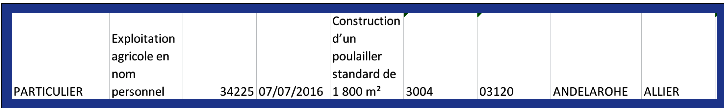
\includegraphics[width=\textwidth]{images/anonymisation/exemple1_anonymisation.png}
    \caption{Enregistrement dans base de données publique}
    \label{fig:Enregistrement dans base de données publique}
\end{figure}
Après quelque recherche sur un moteur de recherche, en utilisant les mots clés poulailler, Allier, 1800\begin{math}m^{2}\end{math} j'ai trouver deux articles de journal qui en parler et à partir de là j'ai pu identifier la personne propriétaire du poulailler.
\begin {figure}
\begin{center}
    \hbox{ 
    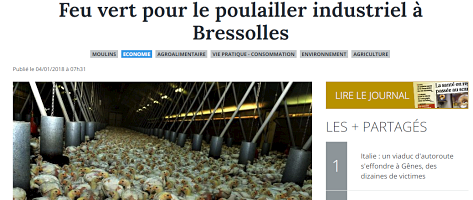
\includegraphics[height=3cm]{images/anonymisation/exemple2_anonymisation.png}
    \hspace*{1cm}  %% pour mettre un espace (horizontal) de 5cm entre les deux images
    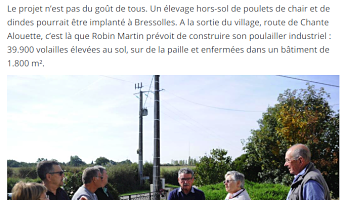
\includegraphics[height=3cm]{images/anonymisation/exemple3_anonymisation.png}
  }
\caption{Articles de Journal}
\label{fig : Articles de Journal}
\end{center}
\end {figure}

Dans l'exemple précèdent, on remarque à quel point il peut être parfois facile de ré-identifier une personne à partir de données publiques. Dans la suite de ce rapport, j'essaye de transposé  les techniques d'anonymisation vues précédemment sur des données à caractères agronomique en se focalisant surtout sur la dimension spatiale des données car la dimension temporelle peut être facilement masquer. Le but étant de conserver l'utilité des données.

%%%%%%%%%%% GÉNÉRALISATION %%%%%%%%%%%
\section{La Généralisation}
L' approche la plus couramment utilisée pour rendre anonyme des données géographique est la généralisation. Elle se rapporte à la technique de généralisation vue plus haut. Elle consiste à réduire la précision au niveau géographique. On crée ainsi de classe d’équivalence, avec des enregistrements ayant une localisation spatiale identique. Selon la clarté sur les données et le niveau de sécurité que l’on souhaite, la réduction de la précision géographique peut être utilisé pour contrôler la taille des classes d’équivalence. Deux techniques ressortent parmi les techniques de généralisation:  
\begin{itemize}
    \item Le Changement d’échelle : cette approche consiste à réduire la précision géographique en élargissant les zones visées par les attributs géographiques. Le changement d'échelle peut s'obtenir de plusieurs façon : \begin{itemize}
        \item  On peut supprimer les trois derniers chiffres des codes postaux, se référent à une grande zone géographique.
        \item   Les coordonnées GPS peuvent être remplacé par le nom de la commune, de la région ou du canton.
    \end{itemize} 
    Le changement d’échelle est donc tout simplement une application du k-anonymat sur des données géographiques. 
    \item   Le Carroyage : Le carroyage est une technique de quadrillage utilisée en topographie, afin de rassembler et de traiter des données en vue d’une exploitation cartographique ou statistique. Il est très similaire au changement d’échelle à l’exception que pour celui-ci, toutes les subdivisions sont de même taille ce qui n’est pas le cas pour changement d’échelle. 
\end{itemize}

%%%%%%%%%%% Génération des données %%%%%%%%%%%
\section{La Génération des données}
Une autre approche serait la génération des données. C'est-à-dire qu'a partir d'un certain jeu de données, on pourrait en générer un autre en ajoutant ou en supprimant de l'information. Cela reviendrait à appliquer la technique de l'ajout de bruit.Il resterait alors à surmonter la difficulté de rendre cohérent les données ainsi générées. En effet, Comme vu précédemment, l'ajout de bruit est souvent confronter à deux problèmes : soit le bruit n'est pas suffisant et dans ce cas l'anonymisation n'est pas efficace, soit il y a beaucoup de bruit et la données perd son utilité.
%%%%%%%%%%% Déplacement des Coordonnées %%%%%%%%%%%
\section{Déplacement des coordonnées}
 La dernière approche pour qui peut être utiliser sur des coordonnées spatiales consisterait à faire une permutation(brouillage) des coordonnées. Il faudra cependant respecter certaines contraintes pour garder la cohérence des données ainsi que leur utilité. Exemples : 
 \begin{itemize}
     \item deux points de coordonnées proches avant le brouillage, doivent l'être aussi après le brouillage
     \item brouiller les coordonnées de façon uniforme dans chaque zone Figure \ref{fig:Brouillage uniforme}
     \item Mais si par exemple la station météo la plus proche d’une parcelle de la zone A se trouve dans la zone B, alors brouiller les coordonnées en tenant compte du voisinage. Figure \ref{fig:Brouillage avec gestion de voisinage}
 \end{itemize}
 
 \begin{figure}[!h]
    \centering
    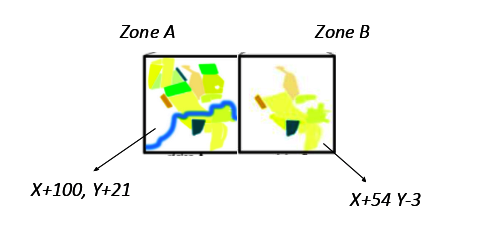
\includegraphics[width=.5\textwidth]{images/anonymisation/brouillage_image1.png}
    \caption{ brouillage uniforme}
    \label{fig:Brouillage uniforme}
\end{figure}
\begin{figure}[!h]
    \centering
    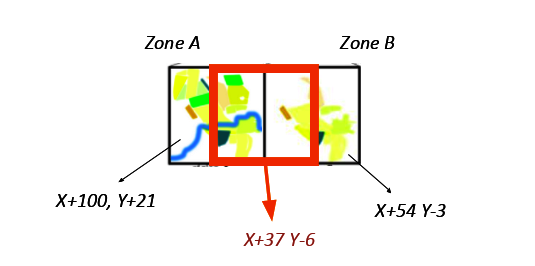
\includegraphics[width=.5\textwidth]{images/anonymisation/brouillage_image2.png}
    \caption{ Brouillage avec gestion de voisinage}
    \label{fig:Brouillage avec gestion de voisinage}
\end{figure}

\chapter{Conclusion}
Compte tenu de la réglementation actuelle, il y a obligation d'assurer une  confidentialité minimale  des données en général et des données à caractères personnelles en particulier. Il existe plusieurs méthodes et techniques qui assurent cette confidentialité mais le choix de celles-ci dépendra de la sensibilité des données ou des applications visées. Ce choix dépendra aussi de l'ensemble des moyens (techniques et financiers) raisonnablement susceptible d'être utilisé pour identifier une personne physique directement ou indirectement. Bien que le domaine agricole soit en retard par rapport au monde de la santé et de la finance en matière de protection des données, il est essentiel que celui-ci puisse vite se développer pour renforcer la confiance des producteurs nécessaire aux partages de leurs données et permettre ainsi de faire émerger de nouvelles connaissances et de nouveaux services.
    \renewcommand{\partname}{}
\renewcommand{\chaptername}{}
\renewcommand{\thechapter}{}
\renewcommand{\thesection}{}

\part{Bilan}
    
  \bibliographystyle{abbrv}
\bibliography{Annexes/biblio}

    %annexes
    \appendix
    \part{Annexes}
    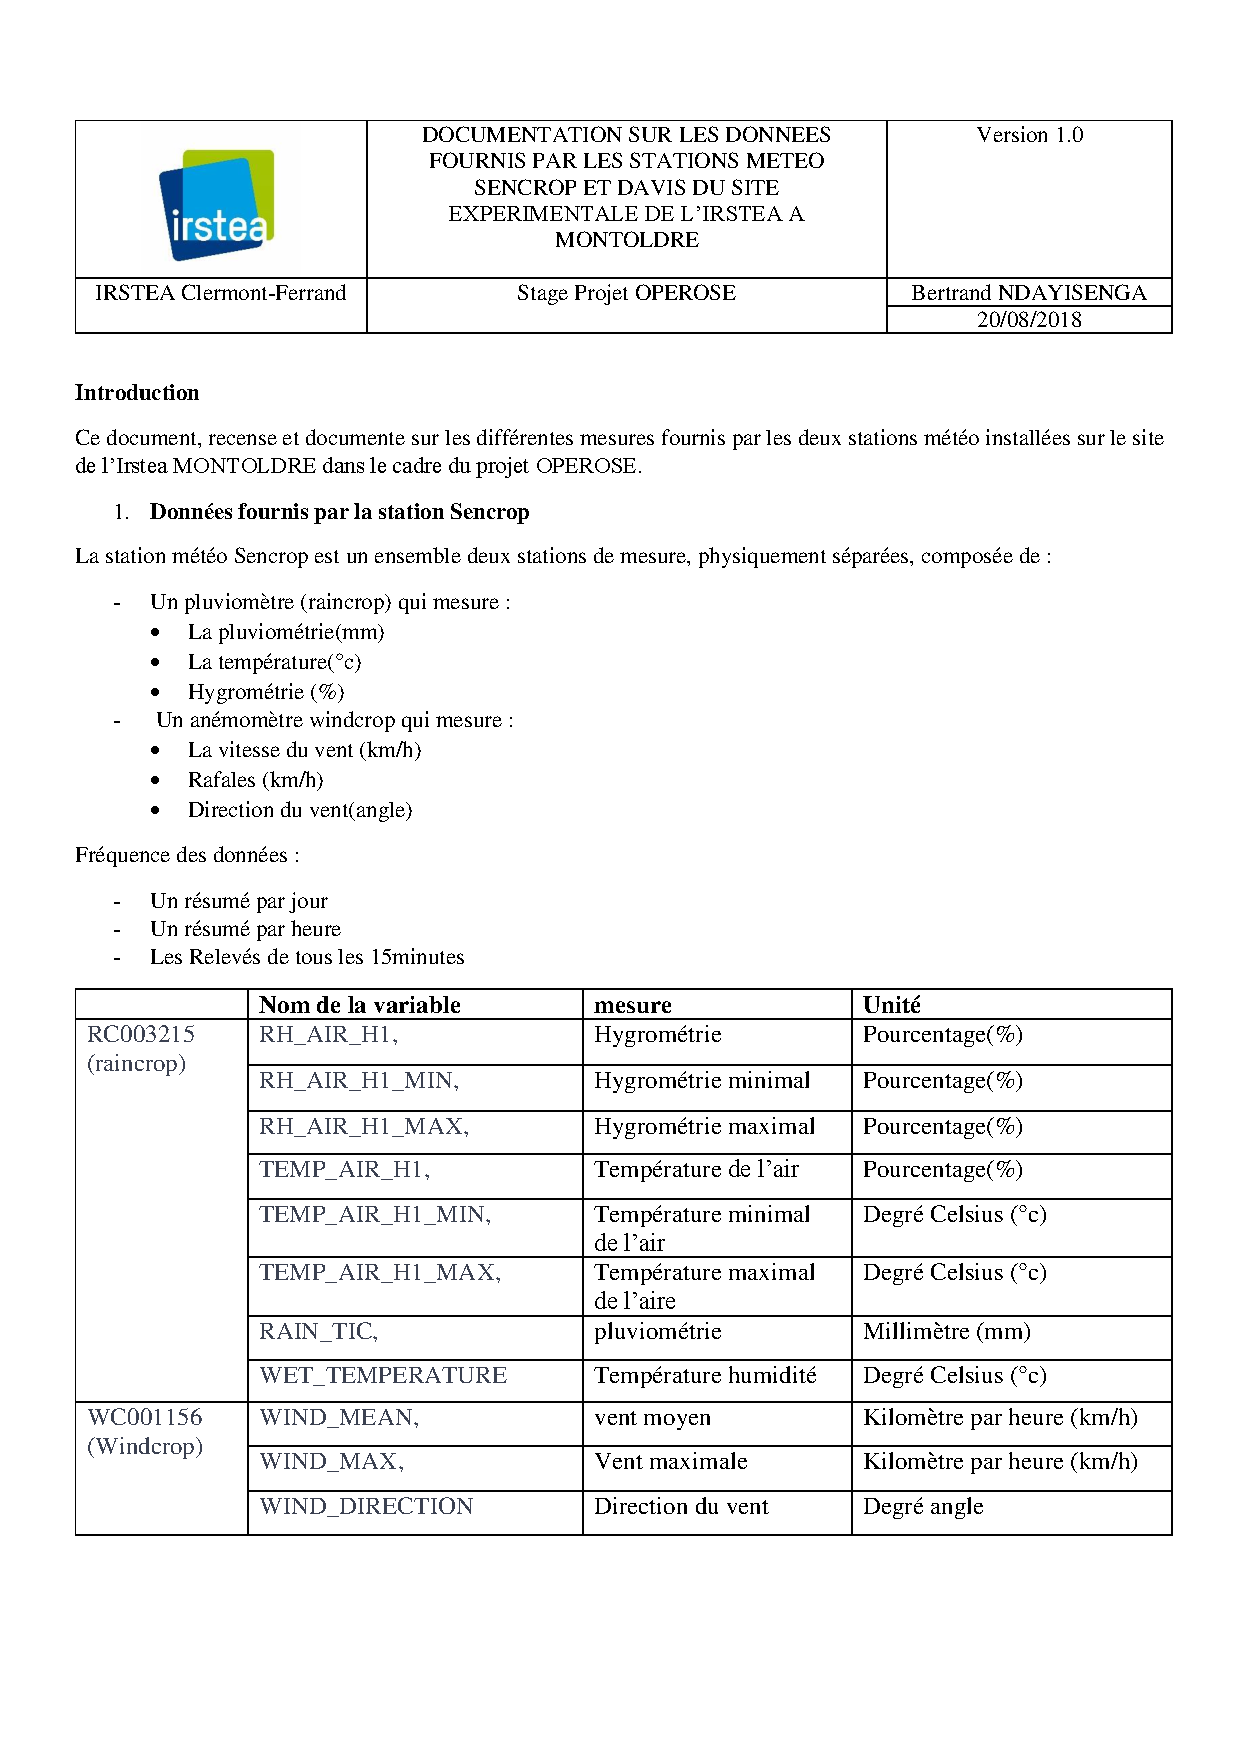
\includepdf[pages={1-3}]{pdfFiles/documentations.pdf}
    
\end{document}          